%% LyX 2.0.4 created this file.  For more info, see http://www.lyx.org/.
%% Do not edit unless you really know what you are doing.
\documentclass[oneside,dutch]{amsart}
\usepackage[T1]{fontenc}
\usepackage[latin9]{inputenc}
\usepackage[a4paper]{geometry}
\geometry{verbose,tmargin=3cm,bmargin=3cm,lmargin=2cm,rmargin=2cm}
\setlength{\parskip}{\smallskipamount}
\setlength{\parindent}{0pt}
\usepackage{array}
\usepackage{amsthm}
\usepackage{graphicx}
\graphicspath{{Figures/}}

\makeatletter

%%%%%%%%%%%%%%%%%%%%%%%%%%%%%% LyX specific LaTeX commands.
%% Because html converters don't know tabularnewline
\providecommand{\tabularnewline}{\\}
%% A simple dot to overcome graphicx limitations
\newcommand{\lyxdot}{.}


%%%%%%%%%%%%%%%%%%%%%%%%%%%%%% Textclass specific LaTeX commands.
\numberwithin{equation}{section}
\numberwithin{figure}{section}

\makeatother

\usepackage{babel}
\begin{document}

\title{Het Heelal}


\author{N.G. Schultheiss}

\maketitle

\section{Inleiding}

Deze module volgt op de module ``De hemel''. Deze module wordt vervolgd
met de module ``Meten met een Telescoop''. Uiteindelijk kun je met
de opgedane kennis een telescoop als meetinstrument toepassen. 


\section{De mens als maat der dingen}

Als we om ons heen kijken, zien we de dingen op menselijke maat. De
grootte van deze dingen kunnen we het beste in meter uitdrukken. Zo
zijn een stoel en een tafel ongeveer een meter groot. We kunnen ook
kijken naar grotere of kleinere ``werelden'' dan de wereld op menselijke
maat.

Een poezen of konijnen wereld bevat dingen die globaal 10 keer zo
klein zijn, zoals een etensbakje of een konijnenhok. De grootte van
deze dingen kunnen we beter in decimeter uitdrukken.

In een 10 keer grotere wereld dan de mensen wereld meten we in decameters.Dingen
waar we aan kunnen denken zijn bijvoorbeeld een blok huizen of een
stadsbus.

We kunnen blijkbaar op verschillende schalen om ons heen kijken, hieronder
zie je een overzicht van de schalen die we normaal kunnen zien:

\begin{figure}[h]
\noindent \begin{centering}
\begin{tabular}{|>{\centering}p{5cm}|>{\centering}p{5cm}|>{\centering}p{5cm}|}
\hline 
Eenheid & Voorwerpen & Organismen\tabularnewline
\hline 
\hline 
\multicolumn{1}{|c|}{mm: millimeter} & zandkorrel & \tabularnewline
\hline 
cm: centimeter & gum & vlieg, gras\tabularnewline
\hline 
dm: decimeter & pen, papier & konijn, bloem\tabularnewline
\hline 
m: meter & meubels, fiets & mens, struik\tabularnewline
\hline 
Dm of dam: decameter & huis, stadsbus & walvis, boom\tabularnewline
\hline 
hm: hectometer & straat, schip & \tabularnewline
\hline 
km: kilometer & dorp, stad & \tabularnewline
\hline 
\end{tabular}
\par\end{centering}

\caption{Menselijk waarneembare werelden}
\end{figure}


Als we in de tabel naar beneden gaan, wordt alles ongeveer 10 maal
zo groot. Gaan we een regel omhoog dan wordt alles ongeveer 10 maal
zo klein. Met de tabel kunnen we zien dat afstand van de ene kant
van een dorp of stad naar de ander kant ongeveer 1000000 zandkorreltjes
is. Een 1000000 is dus een tamelijk groot getal.

Verder kunnen we ook dingen vergelijken. De verhouding van de lengte
van een stadsbus ten ozichte van een straat is ongeveer hetzelfde
als de verhouding van een konijn ten opzichte van een mens. Een straat
is ongeveer 10 stadsbussen lang en een mens is ongeveer 10 konijnen
lang.


\paragraph*{Opdracht 1:}

\emph{We kunnen nu ook proberen hoe de verhouding van de lengte van
een pen ten opzichte van een huis is te geven. Maak af:}
\begin{itemize}
\item \emph{De lengte van een pen verhoudt zich tot de lengte van een huis
als een mens tot een ............................ .}
\item \emph{De lengte van een pen verhoudt zich tot de lengte van een huis
als een zandkorrel tot een ............................ .}
\item \emph{De lengte van een pen verhoudt zich tot de lengte van een huis
als een walvis tot een ............................ .}
\end{itemize}

\paragraph*{Opdracht 2:}

\emph{Het grondoppervlak van een dorp wordt bebouwd met huizen. Schat
hoeveel huizen er in een dorp zijn.}

De lengte van een mens ten opzichte van de diameter van een stad is
ongeveer als de diameter van de stad ten opzichte van de diameter
van de Aarde.

De planeten ``wereld'' is dus ongeveer 1000 maal zo groot als de
steden ``wereld''. Aangezien de wereld ook een planeet is kunnen
we het woord ``wereld'' beter vervangen door ``omgeving''. We
krijgen nu de uitspraak: ``De planeten omgeving is ongeveer 1000
maal zo groot als de steden omgeving.''.

Op vergelijkbare wijze kunnen we ook naar kleinere omgevingen kijken.
Als de stap maken van de mensen omgeving naar de omgeving van een
zandkorrel wordt alles 1000 maal zo klein. Als we nog een dergelijke
stap maken, gaan we van een zandkorrel naar een bacterie. Er gaan
dus ongeveer 1000 bacteri�n in de diameter van een zandkorrel. Dit
kunnen we natuurlijk ook in een tabel uitzetten:

\begin{figure}[h]
\noindent \begin{centering}
\begin{tabular}{|>{\centering}p{1.5cm}|c|>{\centering}p{2cm}|>{\centering}p{7.5cm}|}
\hline 
\multicolumn{3}{|>{\centering}p{7.5cm}|}{Eenheid} & Voorwerpen / organismen\tabularnewline
\hline 
\hline 
 &  & $10^{-18}$m & electron, quark\tabularnewline
\hline 
fm & femtometer & $10^{-15}$m & proton, neutron\tabularnewline
\hline 
pm & picometer & $10^{-12}$m & \tabularnewline
\hline 
\textbf{nm} & \textbf{nanometer} & \textbf{$10^{-9}$}m & \textbf{atoom}\tabularnewline
\hline 
\textbf{$\mu$m} & \textbf{micrometer} & \textbf{$10^{-6}$}m & \textbf{bacterie}\tabularnewline
\hline 
\textbf{mm} & \textbf{millimeter} & \textbf{$10^{-3}$}m & \textbf{zandkorrel}\tabularnewline
\hline 
m & meter & $10^{0}$m & mens\tabularnewline
\hline 
km & kilometer & $10^{3}$m & stad\tabularnewline
\hline 
Mm & megameter & $10^{6}$m & planeet\tabularnewline
\hline 
Gm & gigameter & $10^{9}$m & planeet naar maan\tabularnewline
\hline 
Tm & terameter & $10^{12}$m & planeet naar zon\tabularnewline
\hline 
\end{tabular}
\par\end{centering}

\caption{Afstanden binnen het zonnestelsel}
\end{figure}


Let op: In deze tabel wordt de omgeving 1000 maal of $10^{3}$ maal
zo klein als je een regel omhoog gaat en 1000 maal of $10^{3}$ maal
zo groot als je een regel omlaag gaat. Het dikgedrukte stuk was uitgewerkt
in figuur 2.1.


\paragraph*{Opdracht 3:}

\emph{Een bacterie is ongeveer 1000 atomen lang. Schat hoeveel atomen
er in een bacterie zitten.}


\section{Het Zonnestelsel}

Zoals in figuur 2.2 tezien is kunne we met enige moeite de meter als
maat binne het zonnestelsel gebruiken. Meestal gebruiken we binnen
het zonnestelsel een nieuwe maat, de Astronomische Eenheid of AE.
In het Engels wordt dit de Astronomical Unit of AU.

De astronomische eenheid is ongeveer de afstand van de Zon naar de
Aarde en ligt in de buurt van de 0,150Tm. Volgens Wikipedia is de
AE ongeveer 149.597.870.691m ($\pm$ 6 meter).


\paragraph*{Opdracht 4:}

\emph{Zoek op hoe de astronomische eenheid is gevonden en leg uit
hoe nauwkeurig dit experimenteel is uitgezocht. Kan de nauwkeurigheid
van de meting van de afstand van de Zon tot de Aarde worden vergeleken
met de meting van de lengte van een mens waarbij de afwijking bijvoorbeeld
een konijn, een zandkorrel of een atoom is?}

\begin{figure}[h]
\noindent \begin{centering}
\begin{tabular}{|c|c|c|c|}
\hline 
Naam & Diameter {[}km{]} & Afstand tot de Zon {[}AE{]} & Massa t.o.v. de Aarde\tabularnewline
\hline 
\hline 
Zon & 1.392.000 & - & 332.946\tabularnewline
\hline 
Mercurius & 4.800 & 0.39 & 0.1\tabularnewline
\hline 
Venus & 12.104 & 0.72 & 0.9\tabularnewline
\hline 
Aarde & 12.756 & 1 & 1\tabularnewline
\hline 
Mars & 6794 & 1.5 & 0.1\tabularnewline
\hline 
\multicolumn{4}{|c|}{Planetoiden}\tabularnewline
\hline 
Jupiter & 142.984 & 5.2 & 318\tabularnewline
\hline 
Saturnus & 120.536 & 9.5 & 95\tabularnewline
\hline 
Uranus & 51.118 & 19 & 15\tabularnewline
\hline 
Neptunus & 49.572 & 30 & 17\tabularnewline
\hline 
Kuipergordel &  & 30 tot 50 & \tabularnewline
\hline 
Oortwolk &  & 50.000 tot 100.000 & \tabularnewline
\hline 
\end{tabular}
\par\end{centering}

\caption{Het zonnestelsel}
\end{figure}


Een zonnestelsel bestaat uit een ster waarom planeten draaien. De
ster bevat veruit de meeste massa. De Aarde hoort niet bij de reuzenplaneten
Jupiter, Saturnus, Uranus en Neptunus. De massa van de Aarde is dus
bijzonder klein vergeleken met de massa van het zonnestelsel.


\paragraph*{Opdracht 5:}

\emph{Neem aan dat het zonnestelsel ophoudt na de Ooortwolk. Bereken
hoe groot het zonnestelsel is in {[}Tm{]}.}


\paragraph*{Opdracht 6:}

\emph{Bereken hoeveel procent van de massa van zonnestelsel in de
Zon zit.}


\section{De Melkweg}

Als je naar boven kijkt zie je op een onbewolkte avond lichtpuntjes
aan de hemel. Deze lichtpuntjes zijn naast pla\-neten, manen en kometen
ook sterren. Ons zonnestelsel is met de zichtbare sterren een deel
van ons melkwegstelsel. Met een goede telescoop kun je ook andere
melkwegstelsels in het heelal zien.

In hoofdstuk 3 hebben we gezien dat ons melkwegstelsel na de Oortwolk
ophoudt. De afstand tot de Oortwolk en de daarmee de straal van ons
zonnestelsel kunnen we in de volgende astronomische maat meten: het
lichtjaar. Het lichtjaar is de afstand die het licht in 1 jaar aflegt.
Ons melkwegstelsel is een rafelige pannenkoek met een doorsnede van
100000 lichtjaar of 100 kilolichtjaar en dikte van 2000 lichtjaar
of 2 kilolichtjaar.


\paragraph*{Opdracht 7:}

\emph{Bereken de lengte van een lichtjaar in} {[}Tm{]} \emph{als je
weet dat het licht een snelheid van} $c=299792458[\mathrm{m/s}]$
\emph{heeft, dit is ongeveer} $c=300[\mathrm{Mm/s}]$.


\paragraph*{Opdracht 8:}

\emph{Bereken de tijd die het licht nodig heeft om} 1{[}AE{]} \emph{af
te leggen. Hoeveel lichtminuten is een Astromische Eenheid?}

\begin{figure}[h]
\noindent \begin{centering}
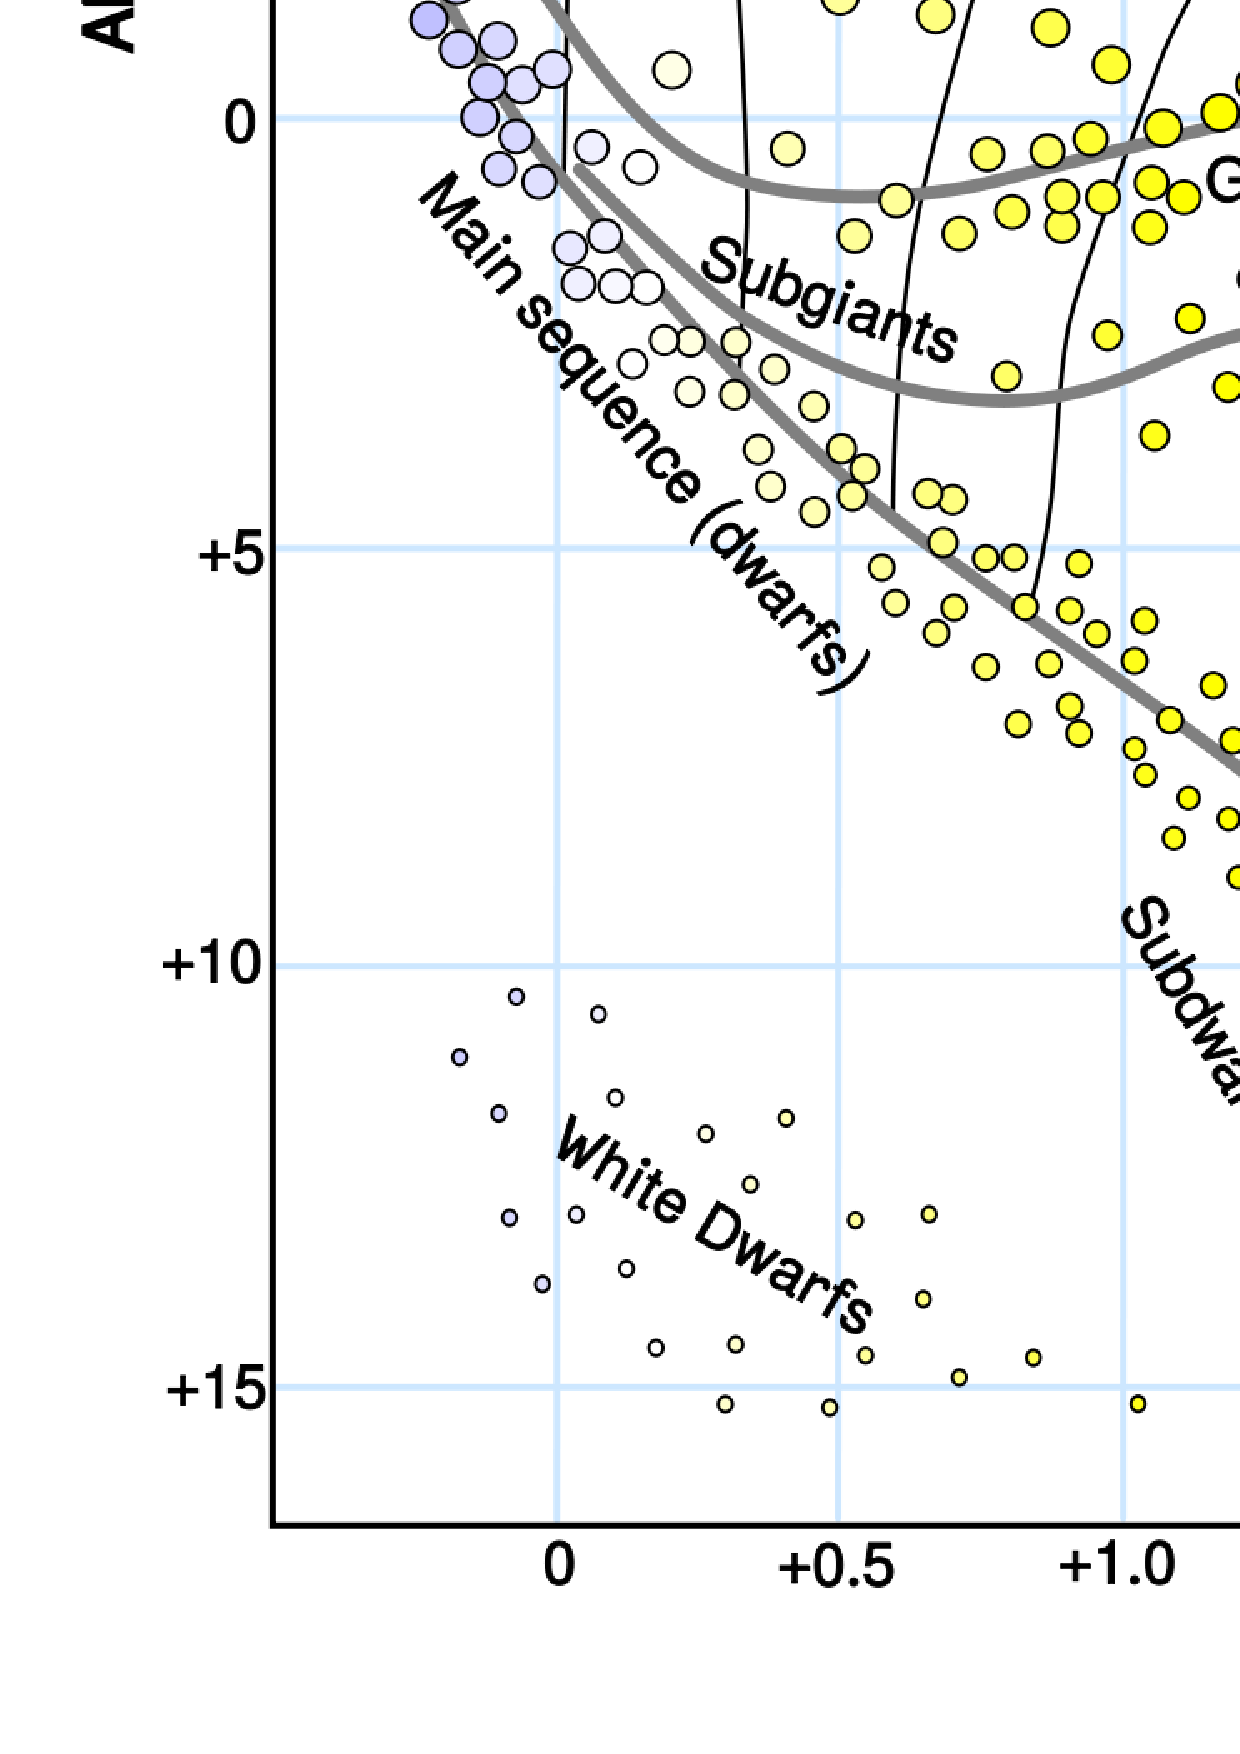
\includegraphics[width=7cm]{H-R_diagram.png}
\par\end{centering}

\caption{Het Hertzsprung-Russell diagram}
\end{figure}


Met een telescoop zijn de sterren aan de hemel natuurlijk te onderzoeken,
dit is onder andere door Ejnar Hertzsprung en Henry Norris Russell
gedaan. Rond 1910 maakten zij het diagram uit figuur 4.1. Dit diagram
is geen sterrenkaart, zoals we in de module ``De Hemel'' hebben
gezien. Hier is de helderheid als absolute magnitude langs de verticale
(x-)as gezet en de kleurindex langs de horizontale (y-)as.


\paragraph*{Opdracht 9:}

\emph{Twee sterren hebben een absolute magnitude van -1 en +5. Leg
uit welke ster het helderst is.}


\paragraph*{Opdracht 10:}

\emph{Een kleurindex van 0 wil zeggen dat een ster een blauwe kleur
heeft. Een kleurindex van 1,5 zegt dat de ster rood is. Leg uit waarom
de sterren globaal van linksboven naar rechtsonder in het Hertzsprung-Russell
diagram gegroepeerd zijn. }

De absolute magnitude is te vinden door de schijnbare magnitude te
corrigeren voor de afstand. Als je verder van een lichtbron bent,
lijkt deze minder helder te worden. Het afnemen van deze helderheid
is met de vogende redenering te vinden:

We vergelijken twee gelijke lichtbronnen A en B.

Lichtbron A doen we in een doos van 1m bij 1m bij 1m. Het licht komt
nu uit alle zijden de doos. Iedere zijde heeft een oppervlak van $1\mathrm{m}^{2}$,
het licht wordt verdeeld over $6\mathrm{m}^{2}$.

Lichtbron B doen we in een doos van 2m bij 2m bij 2m. Het licht komt
ook nu weer uit alle zijden de doos. Iedere zijde heeft een oppervlak
van $4\mathrm{m}^{2}$, het licht wordt verdeeld over $24\mathrm{m}^{2}$.

Het licht van bron B wordt verdeeld over een oppervlak dat 4 maal
zo groot is als het licht van bron A. De gemiddelde helderheid van
bron B lijkt 4 maal zo klein als de gemiddelde helderheid van bron
A. De doos bij bron B was 2 maal zo groot als de doos bij bron A.

We kunnen nu de volgende hypothese formuleren:

\textbf{De schijnbare helderheid is omgekeerd kwadratisch evenredig
met de afstand.}

Dat wil zeggen dat de schijnbare helderheid ``$x^{2}$'' keer zo
klein wordt als de afstand ``$x$'' keer zo groot wordt.


\paragraph*{Opdracht 11: }

\emph{Onderzoek door middel van redeneren of deze hypothese voor een
doos die 3, 4 of 5 keer zo groot is blijft kloppen. Leg uit of je
in deze drie gevallen geluk hebt gehad of dat de hypothese in alle
gevallen klopt.}


\paragraph*{Opdracht 12:}

\emph{Vul in: de schijnbare magnitude ....................................................................
met de afstand.}
\end{document}
